\documentclass[a4paper]{report}

%============ Packages ================
\usepackage{graphicx}
\usepackage{amsmath}
\usepackage{listings}
\usepackage{framed}
%============ End Packages =============

%============ Title ================
\title{\textbf{\Huge{libxmlquery}}\\A lightweight library to query and manipulate XML files}
\author{
Vasco Fernandes\\
MEIC-T, 53801\\
vasco.fernandes@ist.utl.pt \\
\and
Frederico Gon\c{c}alves\\
MEIC-T, 57843\\
frederico.goncalves@ist.utl.pt\\
}
%============ End Title =============

%============ Document ============
\begin{document}

\maketitle

\tableofcontents

%Intro%
\chapter{Introduction}

\section{Motivation} %O google taduz domótica para Home Automation.....%
	As computers tend to get smaller and more powerful, ubiquitous environments begin to emerge as possible and reliable systems. One of the main characteristics of an ubiquitous environment is the fact that it is filled with 
	devices that interoperate in order to provide the user with different kind of services. Home Automation is part of the ubiquitous computing philosophy, in the sense that it fills a certain space with devices that work together in 
	order to provide users with services that are home oriented. Each device has its own characteristics, like a certain operating system, communication medium (Bluetooth, Wifi, etethernet, etc.) and protocols and 
	computational 	capacity. This creates a problem in terms of communication between devices, because each one will communicate with different methods and rules for treating data. This problem stands even if the devices 
	are of equal characteristics, because there are several different software and hardware configurations that can have an effect on data transmission and handling.
	
	We need a system that provides communication between devices and lets us handle the transmitted data with great ease.
	
\section{Problem description}
	When targeting systems built for Home Automation and as said before, we expect a highly heterogeneous environment. One possible solution for this problem is to agree in a common representation and treating method
	for transmitted data. 
	
	Such can be achieved by using XML (e\textbf{X}tensible \textbf{M}arkup \textbf{L}anguage). There are several solutions that use this approach, however they tend to be implemented in languages not suitable for 
	embedded systems. Such solutions also provide a mechanism to query the XML documents, but yet again they're too heavy for embedded systems. We need a lightweight solution that parses and queries XML 
	documents with good degree of performance in embedded systems.
	
	Another concern is how easily is to develop some program that parses and manipulates XML. There are three different phases in this kind of program:
	
	\begin{enumerate}
		\item \textbf{Parsing} - Reading an XML document and building a data structure to hold the parsed information.
		\item \textbf{Getting the correct data} - Traverse the data structure and retrieve the correct portion off the XML that needs to be manipulated.
		\item \textbf{Manipulating} - Alter the retrieved structure and save the changes.
	\end{enumerate}
	
	Each of each phase as different levels of complexity but probably the second is the most tiresome. If the right querying engine is provided to gather the data from the data structure, then this phase can actually be speed 		upped. Also, with the right techniques parsing can be done efficiently, without the need to write code to parse different XML documents.
	
\section{Goal}
	The goal is simple, build a lightweight mechanism to parse, query and manipulate XML documents. We've already achieved this goal, we call it libxmlquery.
	
\section{What is libxmlquery?}
	Libxmlquery is a library designed to parse XML files and query them. It also allows manipulation of the xml elements. It is written in C and was tested in three different kind of operating systems - MS-Windows 7, Linux 2.6 
	and MacOSx 10.4. It uses the flex library to implement the parser, but it is not compiled against it, which means that the end system doesn't need to have the flex library. However, it has a strong dependency on the C library
	and won't work on systems that don't have it.\\
	
	
	The rest of this report is organized as follows: in chapter \ref{chap:arch} we outline the design of our architecture, present the main modules (sections \ref{sec:dom}, \ref{sec:parser} and \ref{sec:sels}) and explain the data 
	structure and macros used in them (section \ref{sec:helpers}); in chapter \ref{chap:eval} we present some profiling tests to the memory usage (section \ref{sec:mprof}) and time usage \ref{sec:tprof}; chapter 
	\ref{chap:concl} we present our main conclusions; in the appendix we shows how to compile against our lib (appendix \ref{chap:gcc}), some sample applications (appendix \ref{chap:app}) and the entire libxmlquery 
	documentation (appendix \ref{chap:doc}).
%END Intro%

%Arch%
\chapter{Architecture}\label{chap:arch}
\section{Overview}\label{sec:overview}
	We begin by describing the modules of our implementation. Figure \ref{fig:arch} shows the scheme of libxmlquery. 

	%Figura da arquitectura
	 \begin{figure}[h!]
		\centering
		\label{fig:arch}
		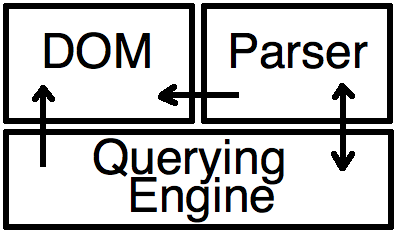
\includegraphics[width=0.5\textwidth] {arch}
		\caption{libxmlquery module design. Three main modules - DOM module responsible for implementing the data structure that holds the xml contents; Parser module, which parses queries and xml documents; 
		Querying engine module, which enables querying to a dom structure.}
	 \end{figure}
	 
	The DOM module defines structures and functions to manipulate a given XML document. As shown in figure \ref{fig:arch}, the DOM module doesn't depend on any other module so it doesn't have to change if any of the 
	others changes. However, if modifications are made to it, then the other modules must change as well, unless the function signature stays exactly the same.
	
	The Parser module is responsible for parsing queries and XML documents. Due to implementation details (see \ref{sec:parser}) we weren't able to separate query parsing from XML parsing. This means that the parser 		depends on both querying engine module and DOM module to work correctly. If any of them changes the parser has to be changed as well. However, if a new parser is needed instead of the one we use, the
	change wouldn't affect the DOM module and the querying engine module would only need one line changed (The line that calls the function, which parses a query). This new parser would only have to build each query 
	and DOM according to each module's interface.
	
	Finally, the query engine module is responsible for parsing queries and querying XML documents. Each query returns a list of the selected elements. Notice that this module depends on both the DOM module and parser 
	module, because it needs to parse queries and use the data structure provided by the DOM module to search the XML document. In a normal use, one would call the query engine module, which would call the parser 
	module and them the DOM module.
	
	We've adopted this architecture in order to support flexibility and modularity. However, the user may need to interact directly with the DOM module, which can be achieve by calling the functions provided by its interface.
	This is also true for the parser module. 
	
	In order to ease the continued development of the library, we've structured the files on disk according to figure \ref{fig:disk}.

	%Figura das pastas em disco.
	 \begin{figure}[h!]
		\centering
		\label{fig:disk}
		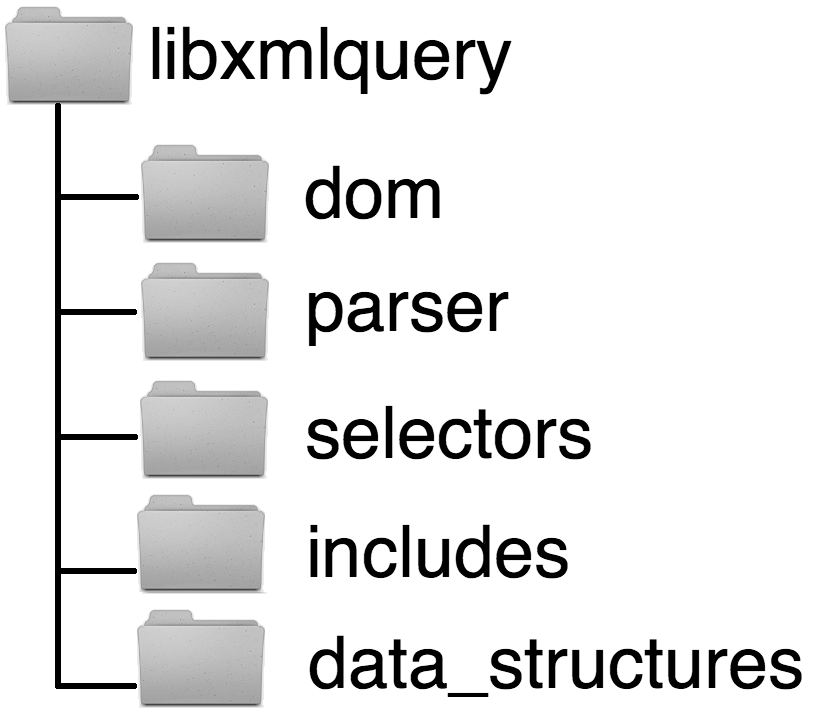
\includegraphics[width=0.30\textwidth] {disk}
		\caption{libxmlquery organization on disk.}
	 \end{figure}
	
	The first two folders are pretty much descriptive, the third one is where all the query engine source code is. The data\_structures folder has various data structures to help us (see section \ref{sec:helpers}) and the includes 
	folder has all the header files of our library.
	
	The next sections detail each module's implementation.

\section{The Document Object Model Module}\label{sec:dom}
	This section describes how our implementation of DOM works. Although DOM is a standard from W3C\footnote{http://www.w3.org/ - Official site of the World Wide Web consortium} we did our own implementation in order 
	to keep it simple and smaller enough for embedded systems. The goal of our DOM implementation is to keep in memory the information stored in the XML file. The idea is to keep the same semantics offered by the XML. In
	order to do this, the DOM creates a tree where every node is either an XML element, attribute, normal text, or CDATA element. Each time an XML document is parsed, the DOM module returns a pointer to its corresponding
	tree root.
	
	\pagebreak
	A tree root is just a structure that holds two pointers. The first one points to what we call XML declaration and the second points to the root element of the XML document. For the sake off better understanding to which each 	structure we're referring, we'll refer to a tree root as a DOM tree. As an example consider the following XML document	:
	
	\lstset{language=XML,caption=Sample XML file, captionpos=b}
	\begin{lstlisting}
		<?xml version="1.0" ?>
		<a>
		   <b />
		</a>
	\end{lstlisting}
	
	The DOM tree returned by the module for this XML contains in its XML declaration pointer the tree corresponding to:
	\lstset{language=XML,caption=Sample XML declaration, captionpos=b}
	\begin{lstlisting}
		<?xml version="1.0" ?>
	\end{lstlisting}
	
	and in its second pointer will have the tree corresponding to:
	\label{lst:xml_example}
	\lstset{language=XML,caption=Sample XML file without XML declaration, captionpos=b}
	\begin{lstlisting}
		<a>
		   <b />
		</a>
	\end{lstlisting}

	Because some documents may not contain the XML declaration part, the DOM will return that pointer pointing to NULL.		

	\subsection{Building the Document Object Module}
		As explained before, the parser module is responsible for constructing the tree returned by the DOM module. It does this by calling upon function provided by the DOM module. Currently, the simplest way of building a 
		DOM tree is to create a new document with the appropriate function and iteratively add all the elements, attributes, normal text and CDATA present in the XML (These functions are described in appendix 
		\ref{chap:doc}).
		
		As a simple example, suppose we would like to parse the XML in \ref{lst:xml_example}. The following code shows how to do this:

	\begin{center}
	\lstset{language=C,numbers=left, captionpos=b, caption=Sample code to build a DOM tree.}
		\begin{tabular}{c}
	\begin{lstlisting}		
...
doc* document = new_document(NULL);
set_doc_root(document, new_element_node("a"));
	
dom_node* root = get_doc_root(document);
append_child(root, new_element_node("b"));
...
	\end{lstlisting}		
	\end{tabular}
	\end{center}
	
		Line 2 creates a DOM tree with no XML declaration. On line 3 we make the root of this tree point to element \textbf{a}. Lines 5 and 6 add element \textbf{b} to the DOM tree and complete the building process.
		
	\subsection{Handling and viewing DOM trees}
		The DOM module also provides functions to retrieve and manipulate the various DOM trees in memory (see appendix \ref{chap:doc}). We strongly recommend the use of \emph{getters} and \emph{setters} to do this,
		because they're deal with implementation detail that shouldn't be dealt by the user.
		
		As the DOM tree gets modified it might help the user if he or she could actually see how it looks like, or save it to disk. This is where serialization comes into play. Currently we support three kinds of serialization - XML; 
		JSON (\textbf{J}ava\textbf{S}cript \textbf{O}bject \textbf{N}otation); YAML (\textbf{Y}AML \textbf{A}in't \textbf{M}arkup \textbf{L}anguage). Serialization is the reverse of parsing, as in it transforms the DOM tree in an XML
		string.
		
	\subsection{Cleaning a document}
		Since our implementation is done in C, there is no garbage collection mechanism. This means that the DOM tree must be freed manually. We provide two functions to do this. One destroys the entire DOM tree the 
		other destroys a generic DOM node (a DOM tree node). However, the second function must be used with care, because it also frees the nodes below the given node.
		
		Freeing up memory space is crucial in an embedded system, but can have a great impact in the systems performance. We leave it to the user to decide where to call these functions.

\section{The Parser Module}\label{sec:parser}
	The parser module implements both the XML parser and the query parser. We've done this because the current implementation is using flex lexical analyzer\footnote{http://flex.sourceforge.net/ - Flex home page.} and 
	bison\footnote{http://dinosaur.compilertools.net/bison/index.html - Bison site} parser generator. One of the biggest disadvantages of flex and bison is that they only support one lexical analyzer per program, which means 
	we may only have one parser built with flex and bison in our library.
	
	Another disadvantage is the fact that we need global variables to store temporally what is parsed with bison. In order to avoid name clashes, each parser global variable has the prefix \textbf{lxq\_} and shouldn't be used 
	directly. Since the parser isn't thread safe, concurrent parsing isn't possible, unless the user ensures that.
	
	Despite of these two disadvantages we've chosen flex and bison because they provide a simple, flexible and extendable way to build very powerful parsers. Moreover, the outcome is a fully optimized parser.
	
	However, the target system doesn't need to have the flex or yaac library. This happens because we're only compiling our library we're not linking it. Since linking does't happen, there is no need to tell the compiler which 
	libraries to use. This method generates and compiles all the code needed for our parser and all functions needed for parsing are in the code. Thus they do not depend on fact of the targeted system having the flex or yacc 
	library.

	\subsection{XML parsing}
		The XML parser implements most of XML features. It is able to parse elements, attributes, normal text and CDATA regions. However, it relies on the fact that the XML had to be validated before parsing began. For this 
		reason, a DOM tree contains only one pointer to the XML root element instead of several pointers to different elements.
	
		Currently we provide two ways of parsing an XML. From a file and from a string, both use the same parsing rules. In fact, there is no difference in them besides the input type.
		
		In order to build the DOM tree the parser needs to interact with it. For this reason, if the DOM module interface changes the parser will have to be modified as well.
	
	\subsection{Query parsing}	
		The query parser implements a parser built for queries compliant to most of the CSS3\footnote{http://www.w3.org/TR/css3-selectors/\#selectors - CSS3 selector list.} standard selectors. We didn't implement every
		selector because they're HTML (\textbf{H}yper\textbf{T}ext \textbf{M}arkup \textbf{L}anguage) specific. For instance, the selector \emph{E:link} selects an element based on the fact that it is a source anchor, which can 
		only happen in HTML files. 
	
		Since querying and XML parsing had to be merge onto a single parser, we had to come up with some kind of distinction between a query and an XML file. We've chosen the character \textbf{@} to indicate that it is a 
		query we're parsing. This means that each query has to be preceded by the character \textbf{@}. As an example consider the following code, which retrieves every element named \textbf{room}.
		
\begin{center}
	\lstset{language=C,numbers=left, captionpos=b, caption=Sample query to a DOM tree.}
		\begin{tabular}{c}
	\begin{lstlisting}		
...
doc* document = parse_xml_from_string("<A> <room /> </A>");
list* query_result = query("@room", get_doc_root(document));
...
	\end{lstlisting}		
	\end{tabular}
	\end{center}
	
		Line 1 parses an XML document from the given string and line 2 queries that document. The result will be an empty element with the tag \textbf{room}. Notice how the query was preceded by \textbf{@}.
			
		Like in XML parsing, the query parser must know the interface of the querying engine module in order to construct the query plan. A query plan is just a sequence of filters that the query engine will apply to the XML
		nodes.
		
\section{The Querying Engine Module}\label{sec:sels}
	This module is responsible for evaluation of the query plan returned by the parser module and its execution. The result of querying an XML document is always a list containing zero or more XML elements. Note that the list
	will contain only elements, it won't return attributes. We'll have to access them through the returned nodes. Nevertheless, querying by attribute is always possible since the querying module is CSS3 compliant.

	The returned list can then be iterated with the proper functions (see section \ref{sec:helpers}).

	One major concern when querying a document is typing the query correctly. Don't forget that the whitespace character is valid in CSS3 and it means \emph{descendants}. For instance, if we want all elements B 
	\emph{descendants} of A we need to write "A B" as a query. In our implementation it becomes "@A B". Since the whitespace character has special meaning, "@A" is different from "@ A". 	
	
	Cleaning up after querying an XML document is very easy. The generated plan is automatically freed by the library, so the user won't have to bother with this part. The only thing that needs to be freed is the returned list of
	results. This list contains pointers to the actual nodes in the DOM tree in order to reduce used memory and enable XML manipulation. This means that the user will only need to destroy the list, leaving the content intact
	(see appendix \ref{chap:doc}).

\section{Data structures and macros}\label{sec:helpers}

	\subsection{Data structures}
		In order to keep the implementation efficient both in time usage and memory usage, we've developed a couple of optimized structures. 
		
		We've built a circular generic list backed up by an array. There are two great features about this list. First it is backed up by an array, which means that elements in the list will be in contiguous memory thus speeding
		up the access. The second great feature is the circular part. Elements in a list can be added and removed as desired. In order to keep a good performance, the list will only grow if necessary. In other words, if the 
		number of elements to keep in the list is much smaller or bigger than its capacity, the list will be resized accordingly.
		
		We've chosen to keep this data structure separated from the rest of the modules because it can hold any type of object, which means it can be used by any code. In particular, it can be used by the user to store its
		own program data.
		
		Since any kind of object can be stored in the list there is no way of type checking each element, so the user must know which elements are present in the list or use another feature of our implementation which is typed 
		elements. Typed element are just simple elements with an integer that indicates their type. For instance, if a list would contain three different types of elements we would encourage the use of typed elements in order 
		to know which kind of data the user is dealing with.
		
		However, they're aren't generic only because they can store any kind of object, but because they implement different policies as well. The user may choose to use the list as a random access list, as a stack, or as a 
		queue. This provides much greater flexibility.
		
		Whichever policy and type of elements the user chooses to use and store, he or she can always iterate over the results by using the appropriate functions (see appendix \ref{doc}). After using an iterator it must be 
		destroyed in order to prevent memory leaks. This is also true for our generic lists. However, in this case we can only free the containers of the list, because we can't possibly know which type of object is stored in each
		one. The user must iterate over the list and free each element one by one. Currently the DOM module and querying engine module use these lists.
		
		Another generic structure we've built is a red black tree. Red black trees are a very good structure when storing unique values that need to be searched. The height of a red black tree is always $\log_2(n)$, where $n$
		is the number of nodes in the tree, thus the search is always done in $\Theta(\log_2(n))$. Currently we use this tree when storing attributes for an XML node.
		
		One concern when developing code that uses this structure is to be careful and don't use the word \emph{RBNIL} for a variable. The red black tree code defines a global variable called RBNIL and uses it with the goal of 
		being efficient.
		
		If the need to iterate over a tree emerges, we've built iterators for this job. There is no guarantee about the order of the returned elements, because the iterator is designed to return every element in the tree with
		only one pass. When iteration is over, the user will have to destroy the iterator (see appendix \ref{chap:doc}. Also, like in the list implementation we provide functions to destroy each tree, but the user must free each
		element stored in each node.
		
	\subsection{Macros}
		This section only describe two macros. The first one is a logging mechanism. We've developed a macro that logs messages with different kind of error levels and supports output formatting. This macro can be found
		almost in any source file we've written. However, it is compilation dependent and when compiled without certain flags it won't get into the binary file (see appendix \ref{chap:gcc}). This helps us debug the code when
		developing and keeps the binary smaller when a final version is created.
		
		The second macro is an allocation macro. The simplest way to describe this macro is to say that its a one line code \emph{malloc} with type cast that exits on allocation failure. In other words, it allocates space and 
		returns a pointer to it, casted to a specific type. If allocation fails, a log message is printed and the program will exit (see appendix \ref{chap:doc}). 

%END Arch%

%Eval%
\chapter{Evaluation}\label{chap:eval}

\section{Test description}\label{sec:testdesc}
	This section presents some tests made to our library. We present only two kinds of tests, that were made in different kinds of systems.\\
	
	The first kind of test is done with a 131986 line XML with 12MB. We're parsing the XML and querying it for a total of 127266 elements. The test was performed on MS-Windows 7, Linux 2.6 and Mac OSx 10.4. Each 
	operating system was running on a 2.6GHz 32-bit intel core duo with 1GB of RAM memory. We've also performed this test on an 250MHz Cavium ARM9 CPU, with 64MB of RAM memory. For each configuration, we've ran 
	the test two times - One without querying engine optimization and other with querying engine optimization. \\
	
	The second test was done with the same configurations, the only difference is that the XML has a total of 36 lines, 0.77KB and we're querying it for 6 elements.\\
	
	Sections \ref{sec:mprof} and \ref{sec:tprof} show the results for these tests. It's important to know that every test was done with a cold cache.
	
\section{Profiling memory usage}\label{sec:mprof}
	This section shows the results for the memory usage on the different systems. The following table shows the result for the first kind of test. Each value is presented in Megabytes and represents the peak usage, that is the 
	maximum amount of memory used.
	
	\begin{center}
  			\begin{tabular}{ | l | r | r | r | r | r | }
			    \hline
				       	       		     			 & Non-optimized (MB) & Optimized (MB)\\ \hline
				    MS-Windows 7   			&  102.23  & 102.23  \\ \hline
				    Linux 2.6 (Intel core duo) 	&  98.78  & 98.78  \\ \hline
				    Linux 2.6 (ARM cpu)   		&  54.2 RAM and 48.58 Swap  & 54.2 RAM and 48.58 Swap \\ \hline
				    Mac OSx 10.4   			&  100.43  & 100.43 \\ 
			    \hline
			\end{tabular}		   
	\end{center}

	From this first test we can already conclude that optimizing the query engine didn't do nothing to optimize space. In fact, further analyzes to our profiling output reveals that the peak memory usage is related to the XML 
	parser. At this point we can't do anything because the parser has already been optimized and the parsed data doesn't have such an overhead. 
	
	In the ARM cpu, since it has only 64MB of RAM, after a while swap area begins to be used. Swapping is done on an SD card with a total of 2GB and a partition of 312MB for swapping. The next table shows the results for 
	the second kind of test.
	
	\begin{center}
  			\begin{tabular}{ | l | r | r | r | r | r | }
			    \hline
				       	       		     			 & Non-optimized (MB) & Optimized (MB)\\ \hline
				    MS-Windows 7   			&  0.035  & 0.035  \\ \hline
				    Linux 2.6 (Intel core duo) 	&  0.026  & 0.026  \\ \hline
				    Linux 2.6 (ARM cpu)   		&  0.030  & 0.030 \\ \hline
				    Mac OSx 10.4   			&  0.032  & 0.032 \\ 
			    \hline
			\end{tabular}		   
	\end{center}
	
	This test confirms that the memory usage peak isn't related with the querying engine. Yet again, a detailed analysis of our profiling output revealed that the peak usage was when data was being parsed.
	
	The results from both tests show that the memory usage depends heavily on the size of the XML and not so much on the number of elements to be queried. We believe that most of XML documents used in Home 
	Automation systems are small, thus not occupying great amounts of memory. That said, the results shows that our solution is adequate for such systems.
	
\section{Time usage}\label{sec:tprof}
	This section shows the time results for each kind of test. The value units are given in seconds. The first table shows the results for the first kind of test.
	
	\begin{center}
  			\begin{tabular}{ | l | r | r | r | r | r | }
			    \hline
				       	       		     			 & Non-optimized (s) & Optimized (s)\\ \hline
				    MS-Windows 7   			&  23.12  & 0.74  \\ \hline
				    Linux 2.6 (Intel core duo) 	&  18.82  & 0.67  \\ \hline
				    Linux 2.6 (ARM cpu)   		&  32.36  & 1.3 \\ \hline
				    Mac OSx 10.4   			&  21.78  & 0.71 \\ 
			    \hline
			\end{tabular}		   
	\end{center}

	This first test shows the impact of query plan evaluation in our design. When optimized the speedup gained is around:
	
		$$speedup = \frac{non-optimized}{optimized} = \frac{18.82}{0.67} = 28.09$$

	In fact, a detailed analysis of our profiling output showed that the non-optimized version wasted to much time on evaluating each query plan. For this reason we've optimized it and show impressive results. The following 
	table shows the results for the second kind of test.
	
	\begin{center}
  			\begin{tabular}{ | l | r | r | r | r | r | }
			    \hline
				       	       		     			 & Non-optimized (s) & Optimized (s)\\ \hline
				    MS-Windows 7   			&  0.003  & $<$ 0.001  \\ \hline
				    Linux 2.6 (Intel core duo) 	&  0.002  & $<$ 0.001  \\ \hline
				    Linux 2.6 (ARM cpu)   		&  0.007  & $<$ 0.001 \\ \hline
				    Mac OSx 10.4   			&  0.002  & $<$ 0.001 \\ 
			    \hline
			\end{tabular}		   
	\end{center}
	
	This test confirms that the query engine optimization was successful. In fact, the optimized version is so fast that there isn't enough granularity to give the precise time it took the program to run.
	
	Another conclusion we take is that memory usage has little impact in time usage. In fact, our profiling output shows that the memory usage peak lasts only during parsing and them drops abruptly. 
%END Eval%

%Conclusion%
\chapter{Conclusion} \label{chap:concl}
	We've presented a solution for an XML library designed for embedded systems. The main goal was to build it as light as possible, while giving the user a flexible and expandable way of parsing, querying and manipulating
	XML documents. 
	
	We've built a library in three modules - A parser module; A DOM module; A querying engine module. Each has its own functionalities and can be modified almost effortlessly.
	
	We've shown that the performance depends heavily on the size of the XML being parsed. Our goal has been reach, as our library provides a flexible way to speedup development of applications that use XML documents
	to store configuration properties.
	 
%END Conclusion%

\appendix 
\chapter{Compiling and using the code}\label{chap:gcc}
	This section shows how to compile our library and compile other programs with our library.
	
	Compiling libxmlquery is very easy. The source code ships with a Makefile, so you just need to type in \emph{make}. On Unix based systems the \emph{make} command comes within the system, on MS-Windows we 
	encourage the use of Cygwin.
	
	When \emph{make} finishes you'll notice a file with the extension \textbf{.so} (Shared Object). You just need to pass this object to the compiler when linking and you're done. You have compiled your program against 
	libxmlquery.
	
	As an example consider the command using \emph{gcc}:
	
	\begin{center}
	\lstset{language=bash,caption=Compiling a program against our library, captionpos=b}
	\begin{tabular}{c}
	\begin{lstlisting}
	gcc -o outputname libxmlquery.so myapplication.c
	\end{lstlisting}
	\end{tabular}
	\end{center}
	
\chapter{Sample applications}\label{chap:app} %lol%
	\section{Shell}
		The application shell is just a simple shell that enable loading XML documents and querying them. Its purpose is just to demonstrate the use of queries. Consider this typical use:

\begin{center}
\lstset{language=bash,caption=Typical usage of the shell application. The banner was intentionally removed., captionpos=b}
\begin{tabular}{c}
\begin{lstlisting}		
>>> load ../test.xml doc
XML ../test.xml loaded and stored in doc
>>> query doc "@room device"
Node:
<device state="on" type="switch" />

Node:
<device state="87" type="blind" />

Node:
<device state="94" type="lights">
  <coord>
    <x>
      205
    </x>
    <y>
      97
    </y>
    <z>
      256
    </z>
  </coord>
</device>

>>> quit
exiting...
\end{lstlisting}
\end{tabular}
\end{center}
		
		In this example, the file \textbf{test.xml} gets loaded into the symbol \textbf{doc}. Then a query is performed on this symbol. It is possible to execute more commands. Type \emph{help} to get a description of them.
		
		The shell application comes with a Makefile, so it's easy to compile it. To compile in other systems see appendix \ref{chap:gcc}.
		
\chapter{Documentation}\label{chap:doc}
	- Docs \\
	
\end{document}